\documentclass[UTF8]{ctexart}
\usepackage{graphicx}
\usepackage{geometry}
\usepackage{float}
\usepackage{diagbox}

\pagestyle{empty}
\geometry{top = 3cm, bottom = 3cm}

\begin{document}
\subsection*{1.}
\paragraph*{(a)} government consumption
\paragraph*{(b)} investment
\paragraph*{(c)} household consumption
\paragraph*{(d)} net export
\paragraph*{(e)} investment
\subsection*{2.}
\subsubsection*{(a)}
In the stage when the farmer sold the wheat to the miller, 500 RMB was added. In the stage of the miller processing the wheat and selling to the baker, 500 RMB was added. When the baker finally sold the bread to the customers, 2000 RMB was added.
\subsubsection*{(b)}
The GDP is 3000 RMB.
\subsection*{3.}
\begin{table}[h]
    \centering
    \begin{tabular}{|c|*{4}{p{14ex}<{\centering}|}}
    \hline
    \diagbox{Year}{Shares} & C & G & I & NX \\ \hline
    \rule{0pt}{16pt} 1980 & 51.47\% & 13.89\% & 34.96\% & -0.32\% \\[6pt] \hline
    \rule{0pt}{16pt} 1990 & 49.74\% & 13.59\% & 33.98\% & 2.69\% \\[6pt] \hline
    \rule{0pt}{16pt} 2000 & 46.96\% & 16.92\% & 33.73\% & 2.39\% \\[6pt] \hline
    \rule{0pt}{16pt} 2010 & 34.63\% & 14.72\% & 46.97\% & 3.69\% \\[6pt] \hline
    \rule{0pt}{16pt} 2018 & 38.67\% & 16.60\% & 43.96\% & 0.77\% \\[6pt] \hline
    \end{tabular}
\end{table}

\subsection*{4.}
\subsubsection*{(a)}
\begin{figure}[H]
    \centering
    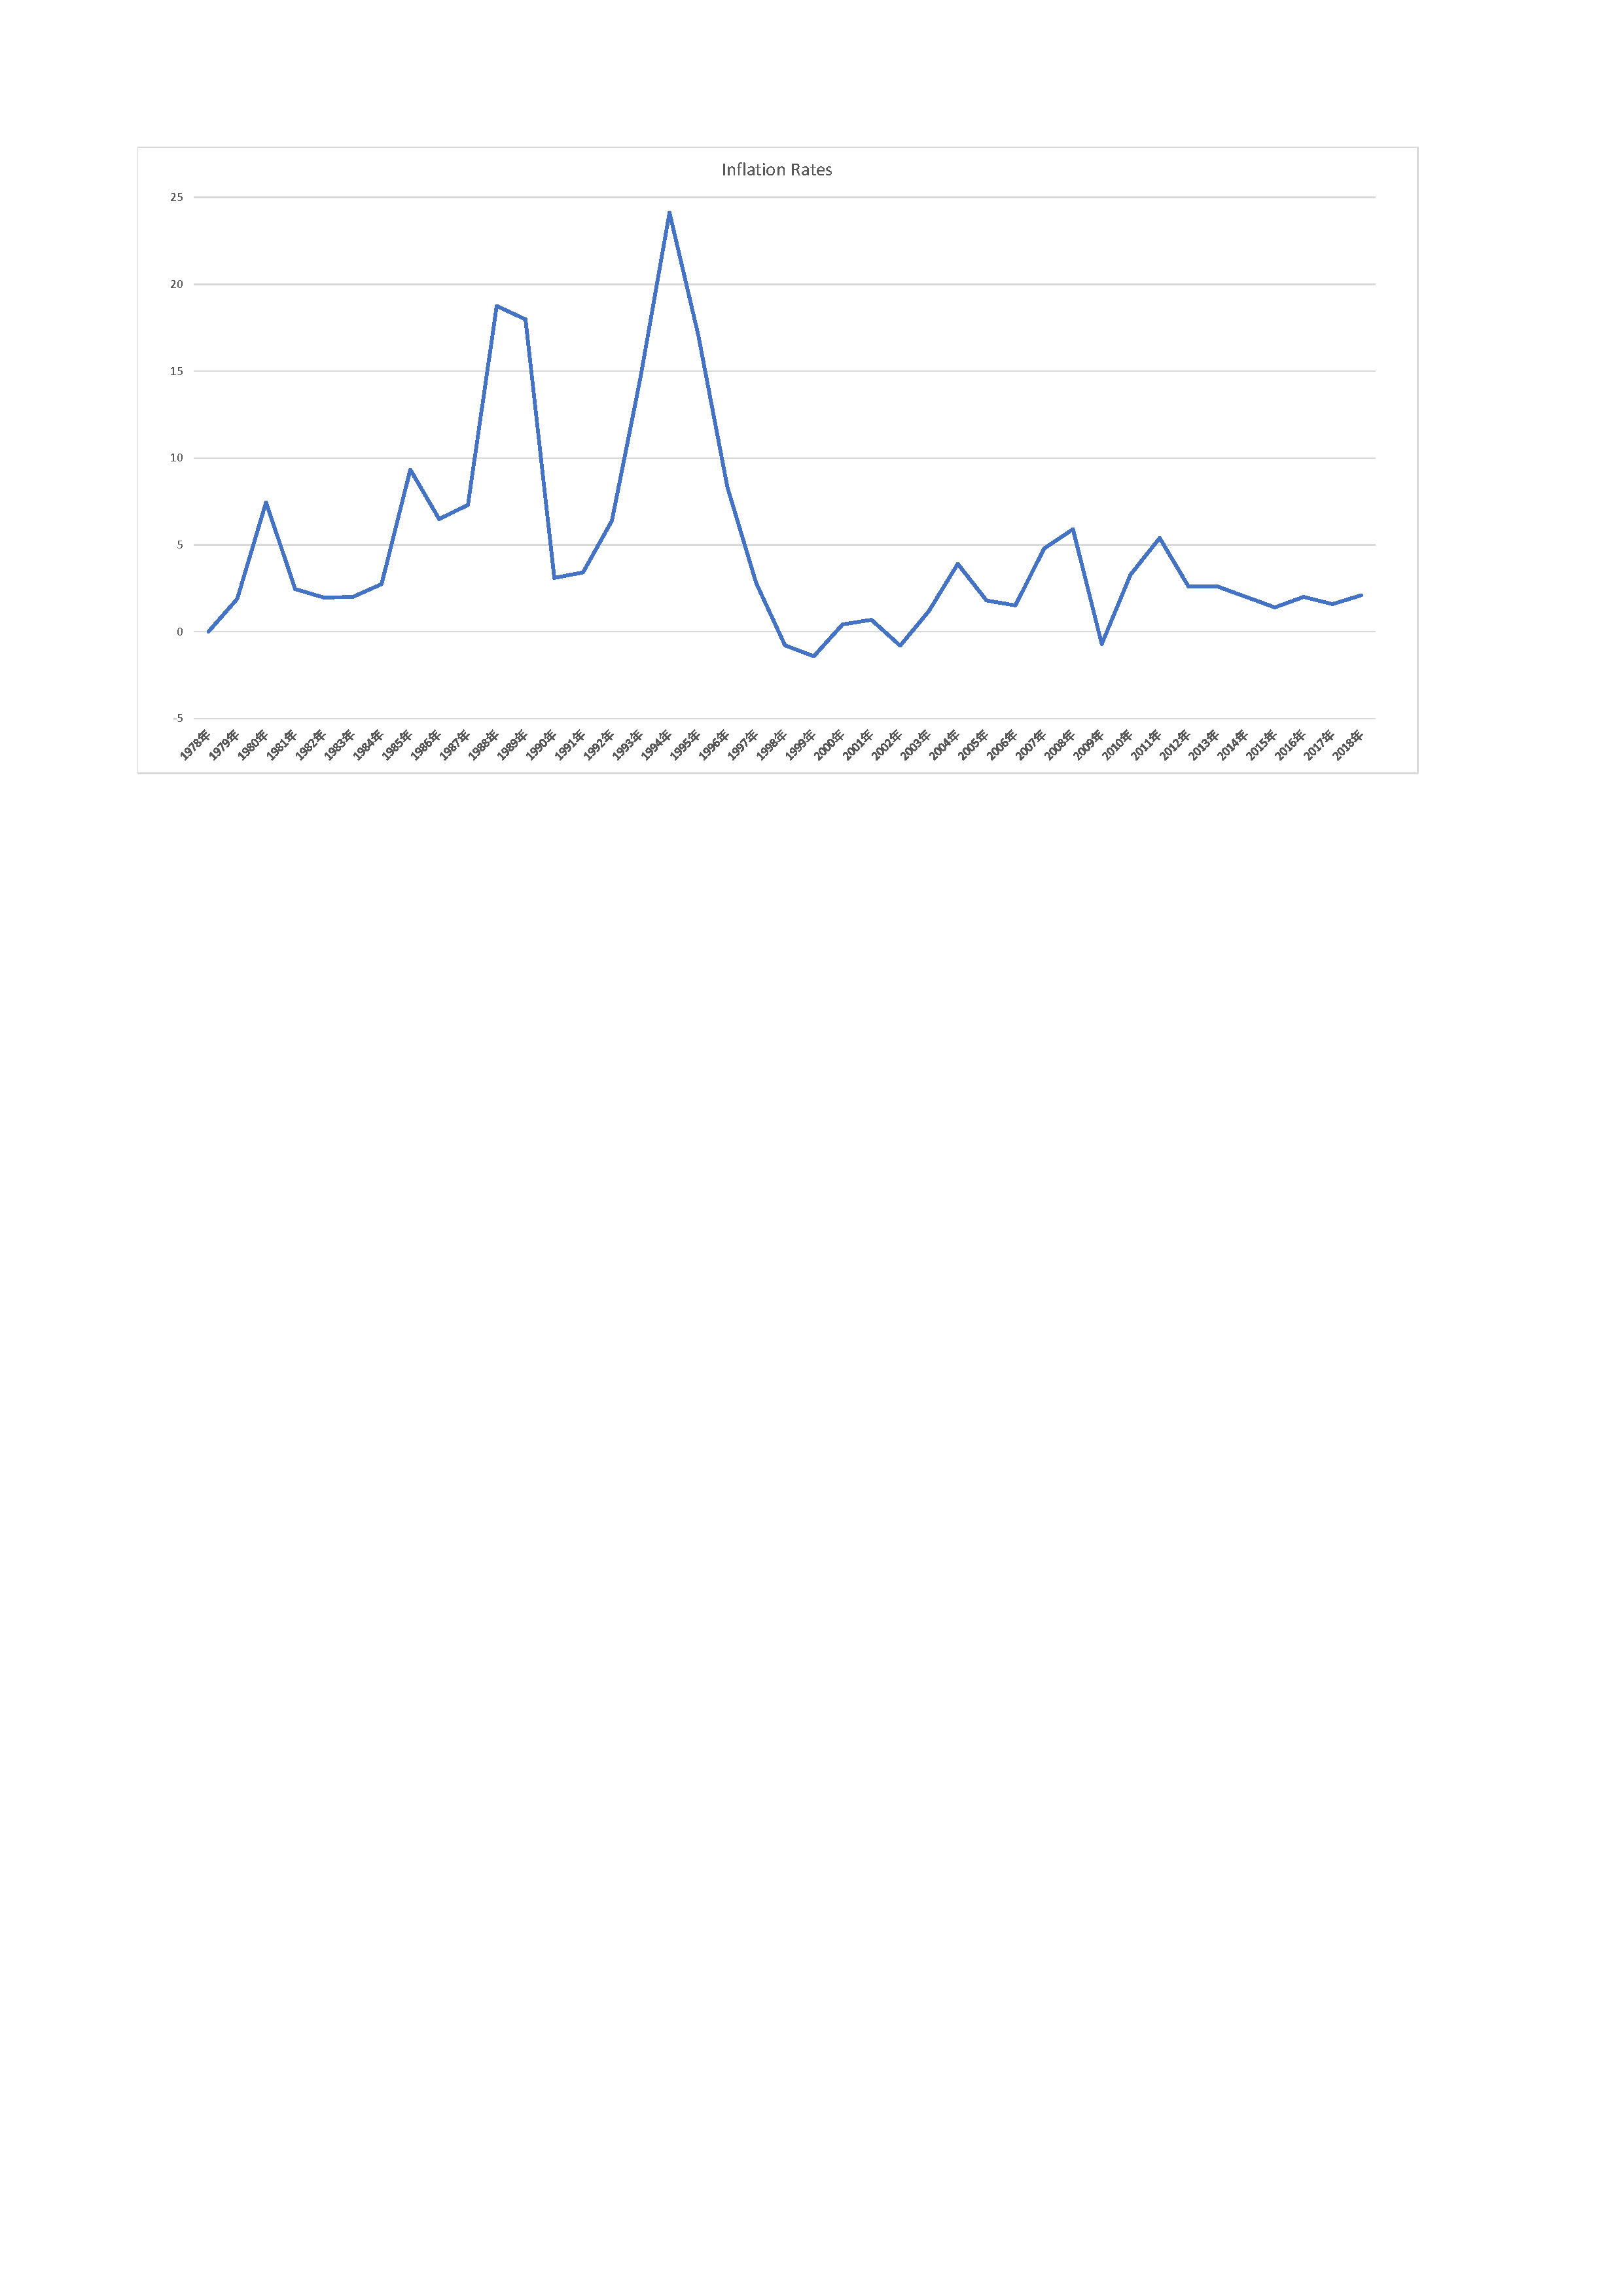
\includegraphics[width=15cm]{Inflation Rates.pdf}
\end{figure}
\subsubsection*{(b)}
\begin{figure}[H]
    \centering
    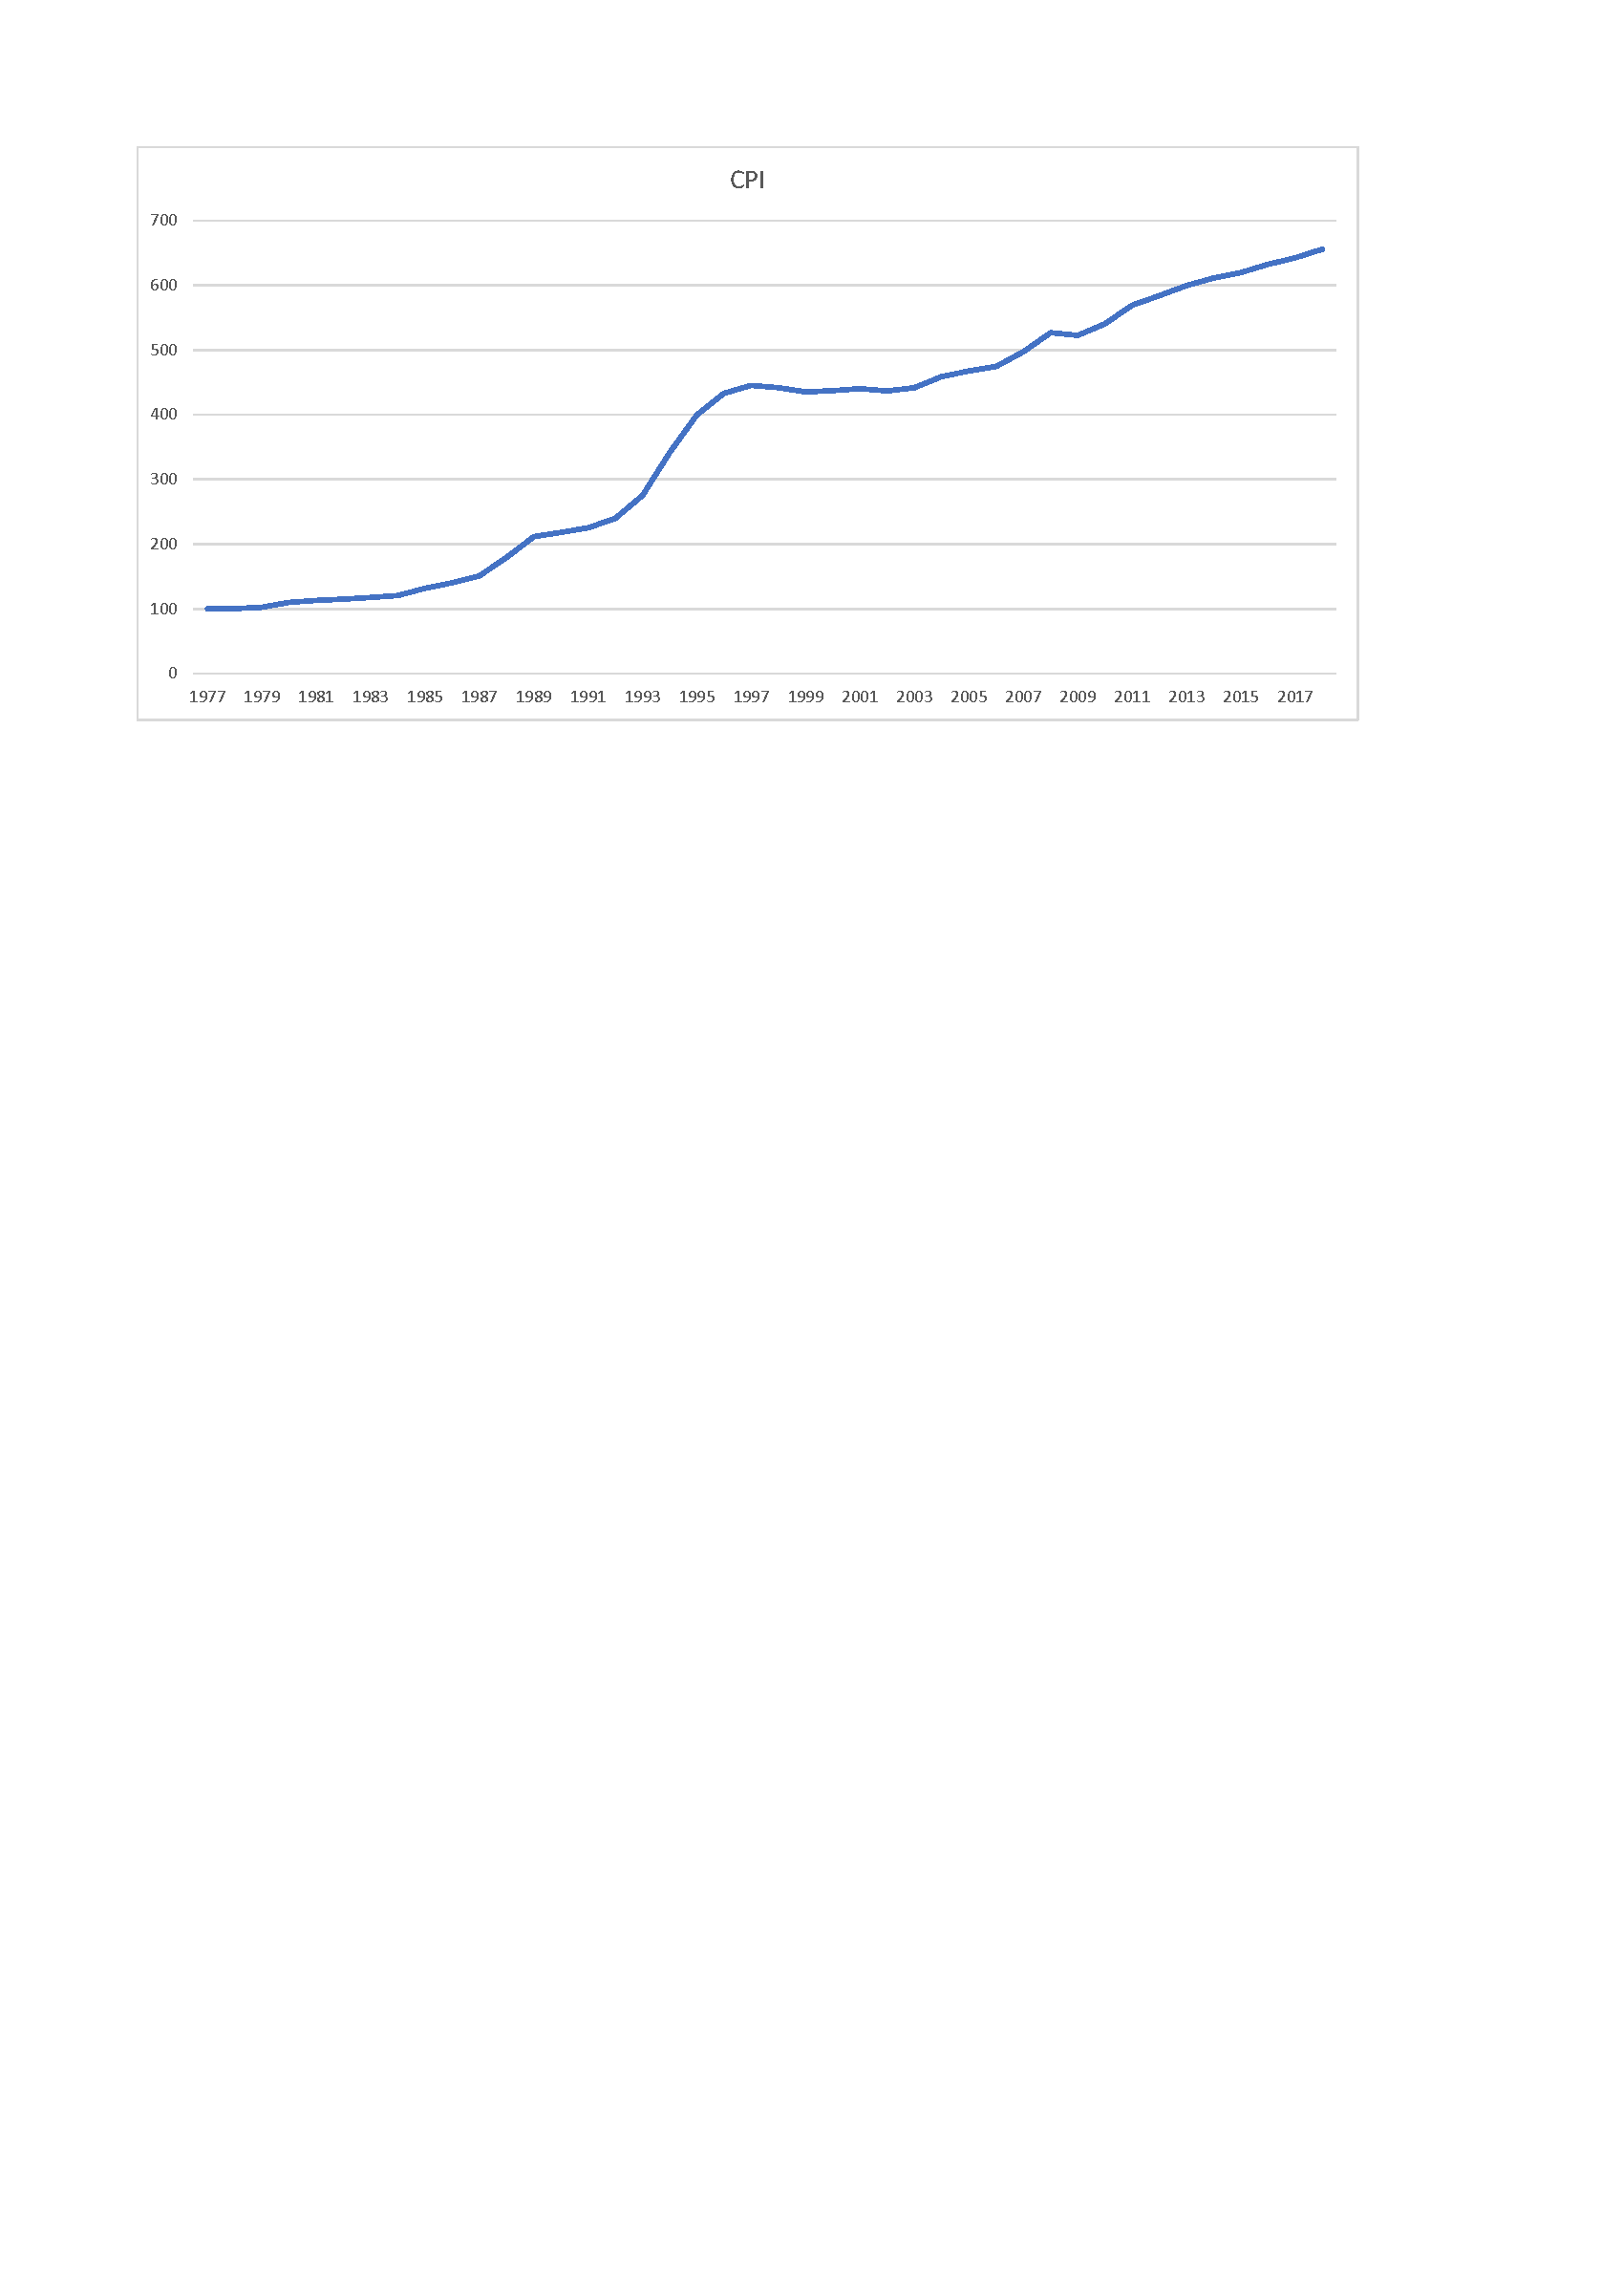
\includegraphics[width=15cm]{CPI.pdf}
\end{figure}
The the general price level in 2018 is more than six times that in in 1977.
\end{document}